\newpage 

\subsection{Task, Data, and Pipeline Parallelism}

Task, data, and pipeline parallelism are three common forms of parallelism:

\begin{Def}[Task Parallelism]

    \textbf{Task parallelism} involves running multiple tasks simultaneously. Each task is independent and can run in parallel with other tasks,
    perhaps even on the same data.
\end{Def}
\noindent
In essence, we may think \underline{same data, different tasks}:
\begin{figure}[h]
    \centering
    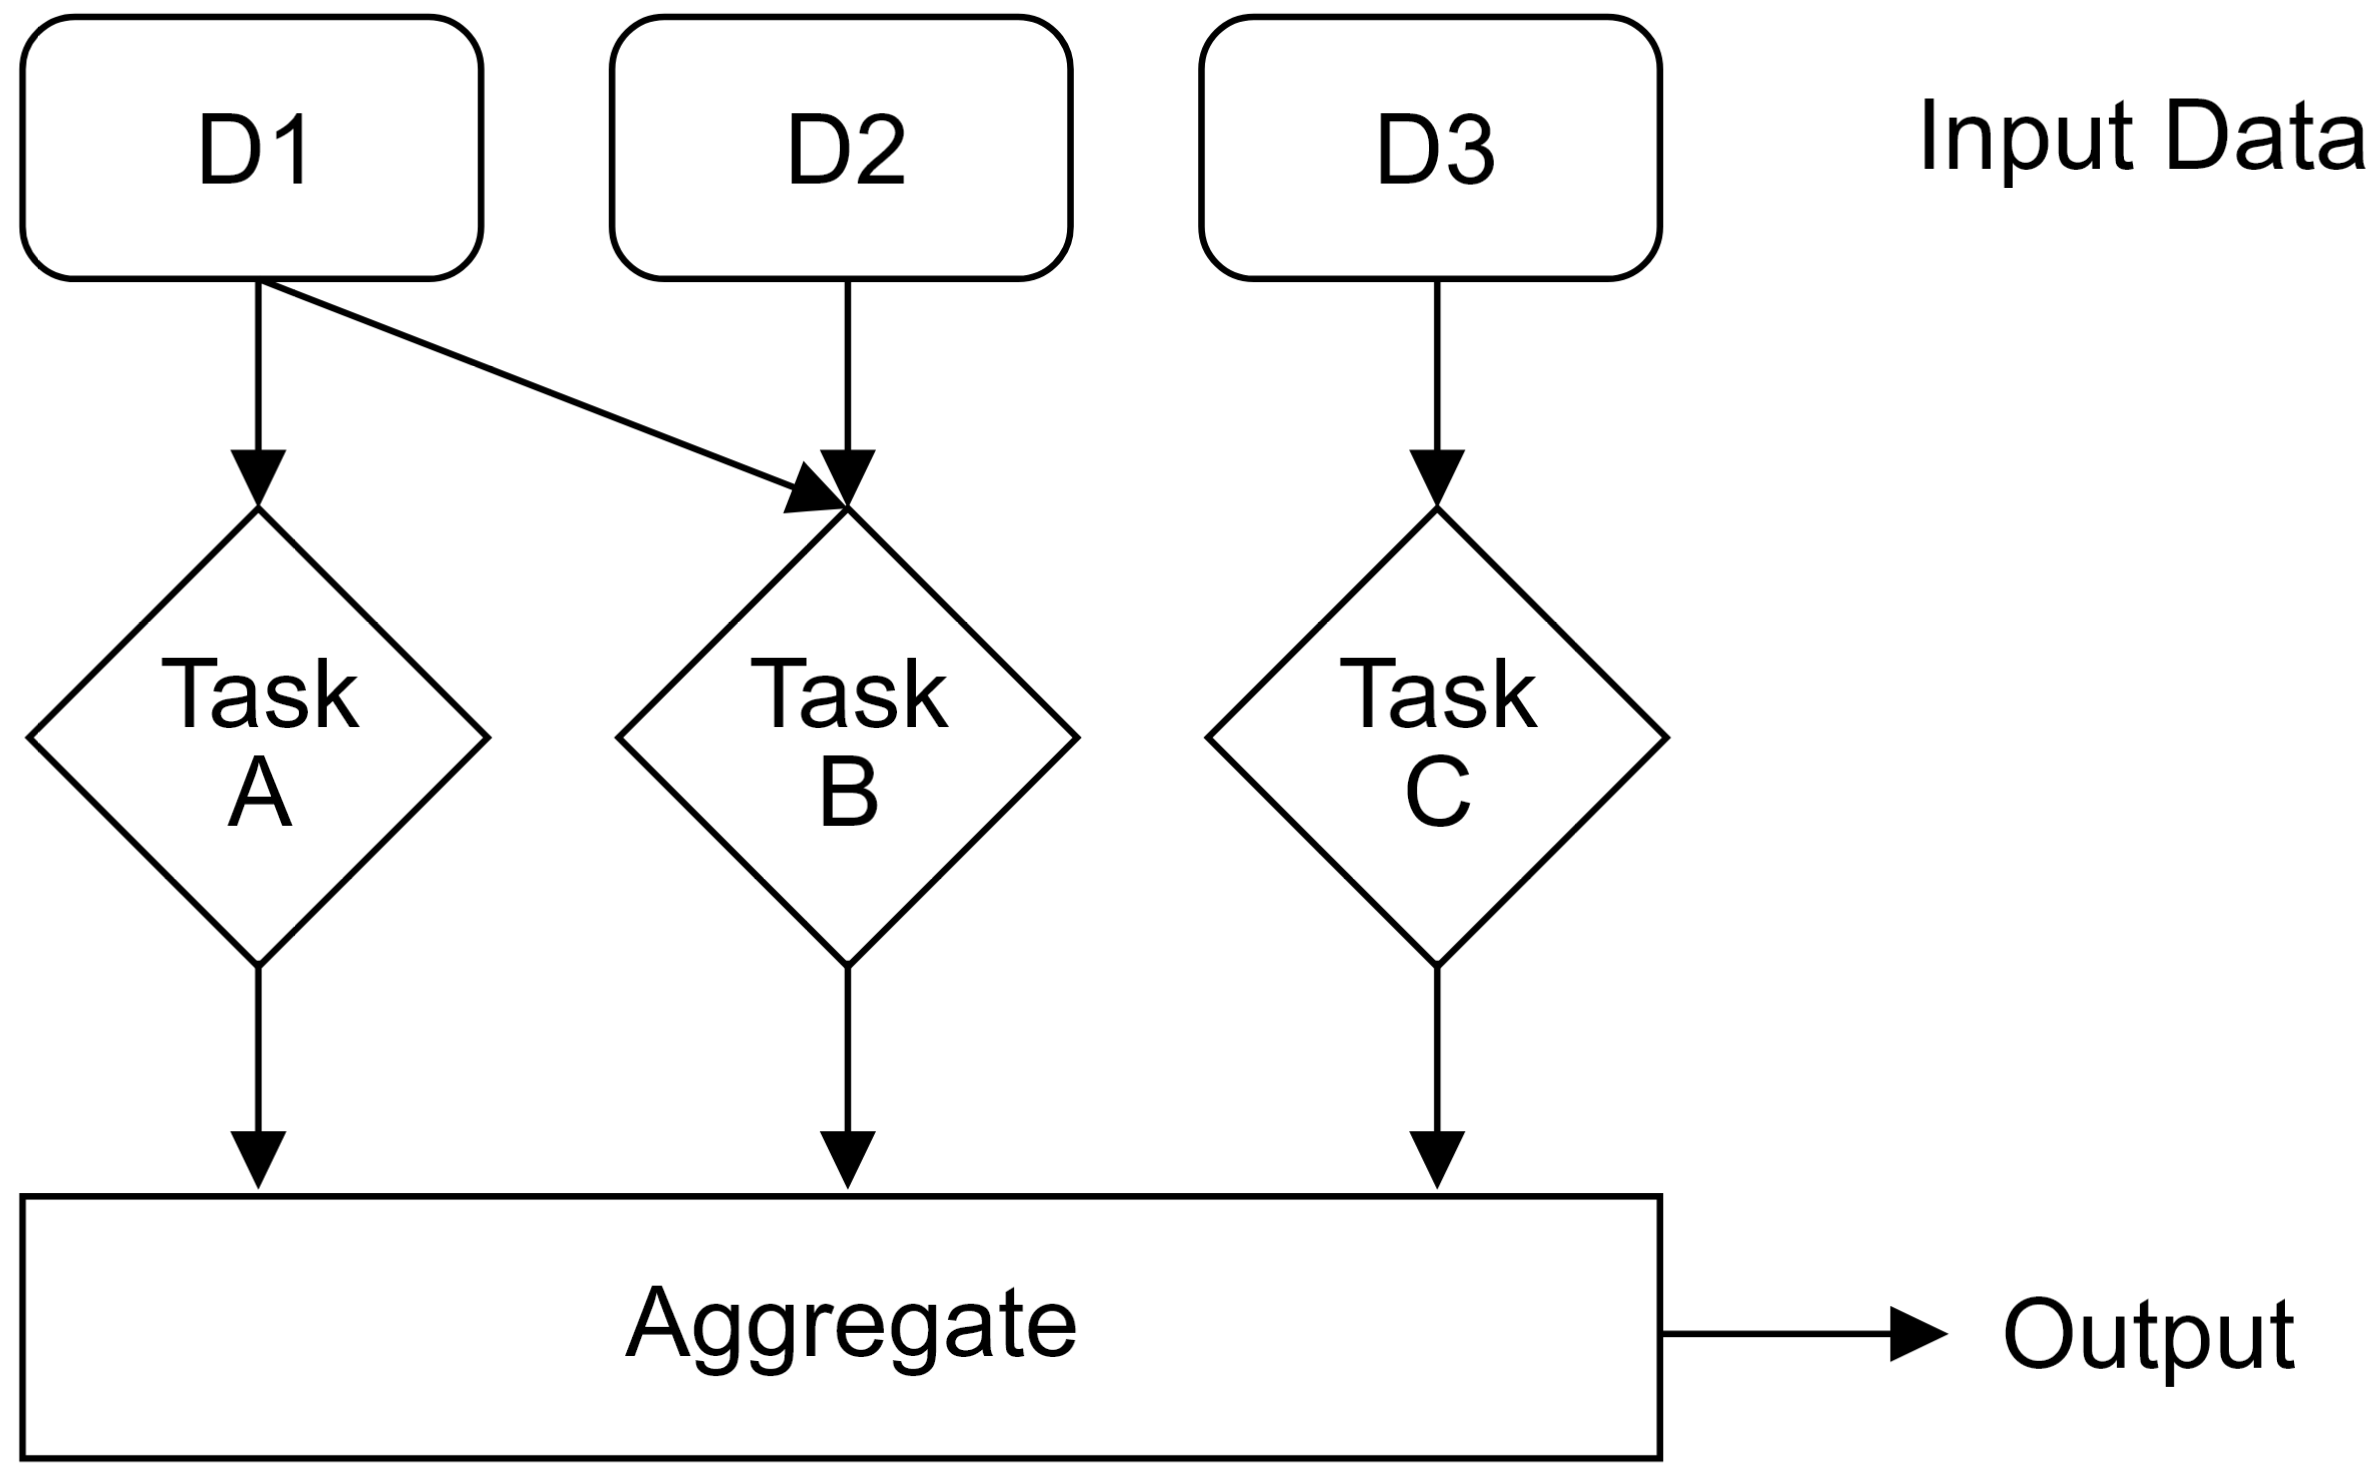
\includegraphics[width=0.5\textwidth]{./Sections/rpc_2/tpar.png}
    \caption{Task Parallelism Culminating into an Aggregate Result}
\end{figure}
\noindent

\vspace{-1em}
\begin{Def}[Data Parallelism]

    \textbf{Data parallelism} involves running the same task on multiple data items. Each task is identical, but the data is different.
\end{Def}
\noindent
We may think \underline{same task, different data}:
\begin{figure}[h]
    \centering
    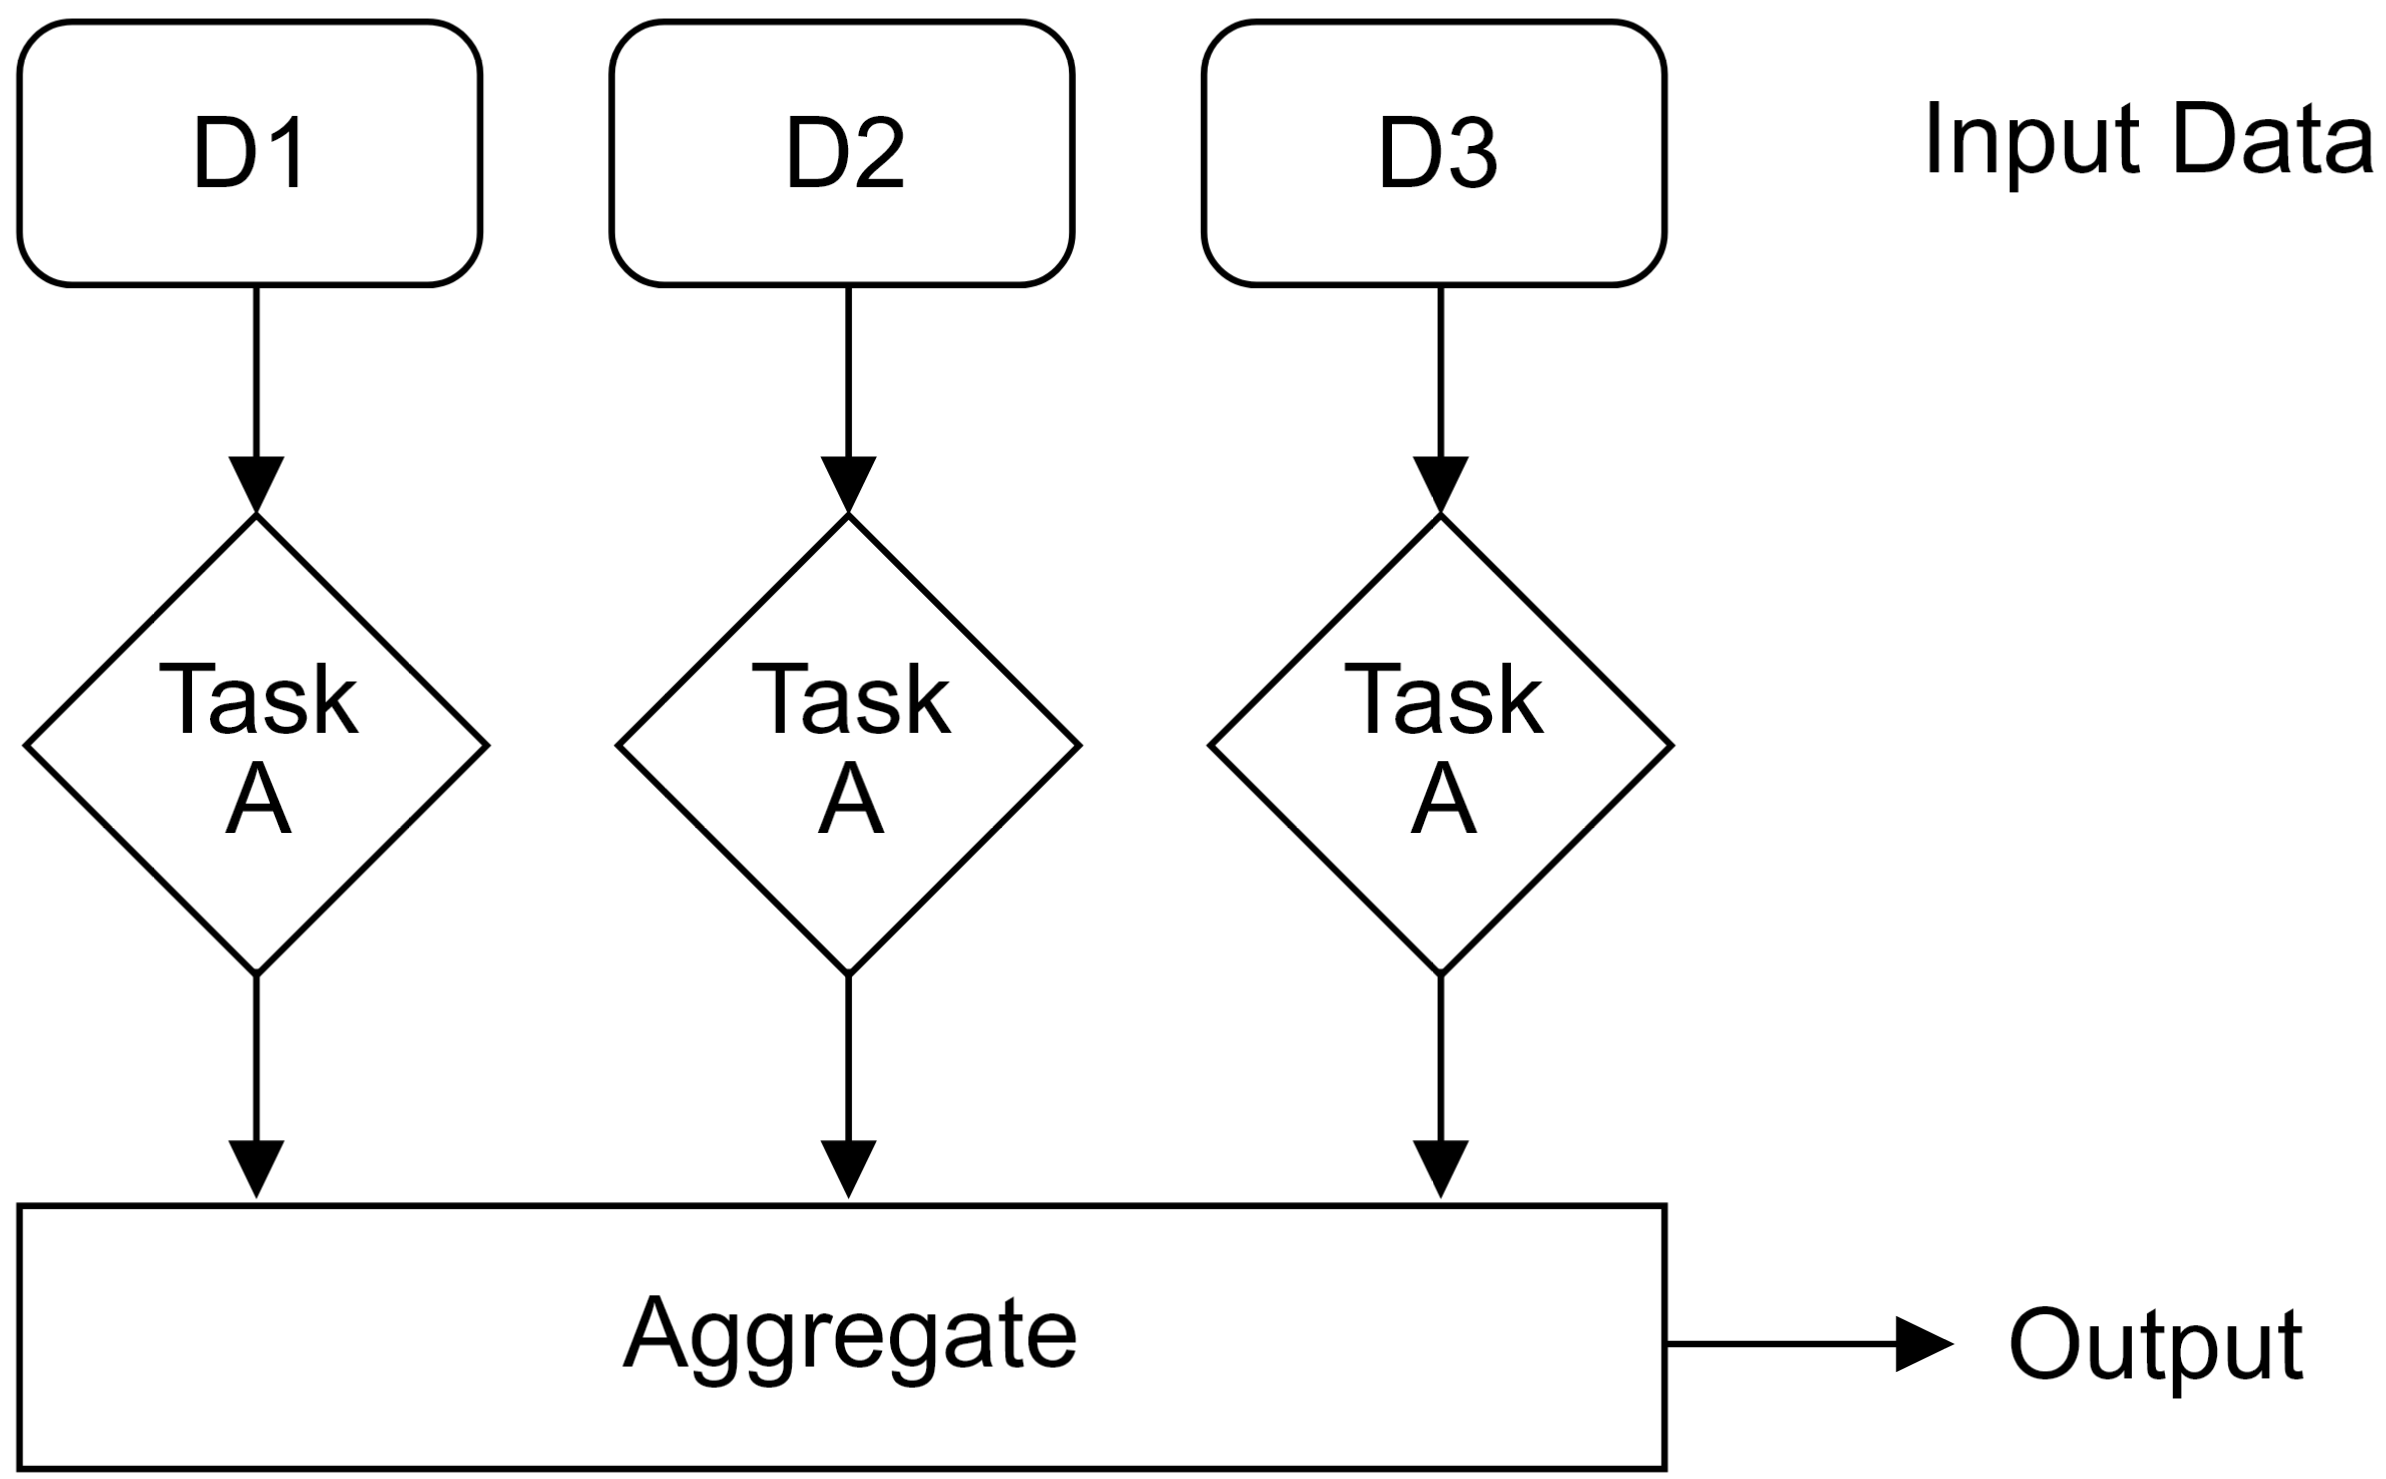
\includegraphics[width=0.5\textwidth]{./Sections/rpc_2/dpar.png}
    \caption{Data Parallelism Culminating into an Aggregate Result}
\end{figure}

\newpage 
\noindent
To continue, we have:
\begin{Def}[Pipeline Parallelism]

    \textbf{Pipeline parallelism} involves breaking a task into multiple stages, each of which can be executed concurrently. The output of one stage is the input to the next stage.
\end{Def}

For instance, consider the following pipeline:
\begin{itemize}
    \item \textbf{Task A}: ``Search for a flight.'' (1 time unit)
    \item \textbf{Task B}: ``Book a flight.'' (1 time unit)
\end{itemize}

\noindent
First consider the scenario where we only have one resource to work with, resulting in concurrency:
\begin{figure}[h]
    \centering
    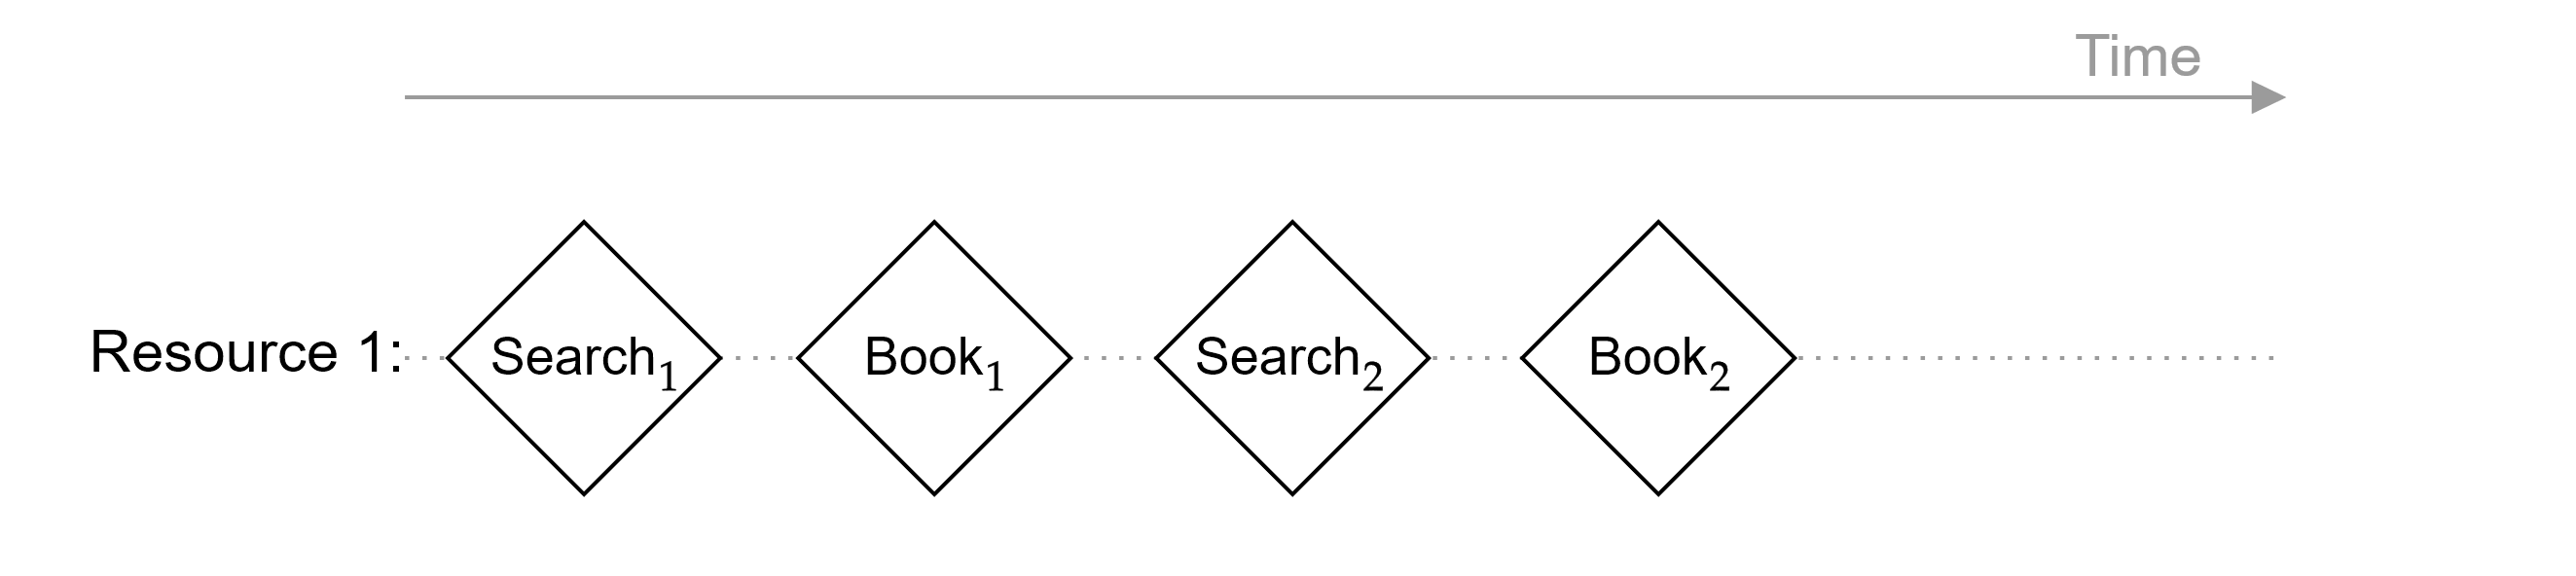
\includegraphics[width=1\textwidth]{./Sections/rpc_2/ppar.png}
    \caption{Searching and Booking flights concurrently}
\end{figure}

\noindent
Now consider the scenario where we have two resources to work with, resulting in parallelism:
\begin{figure}[h]
    \centering
    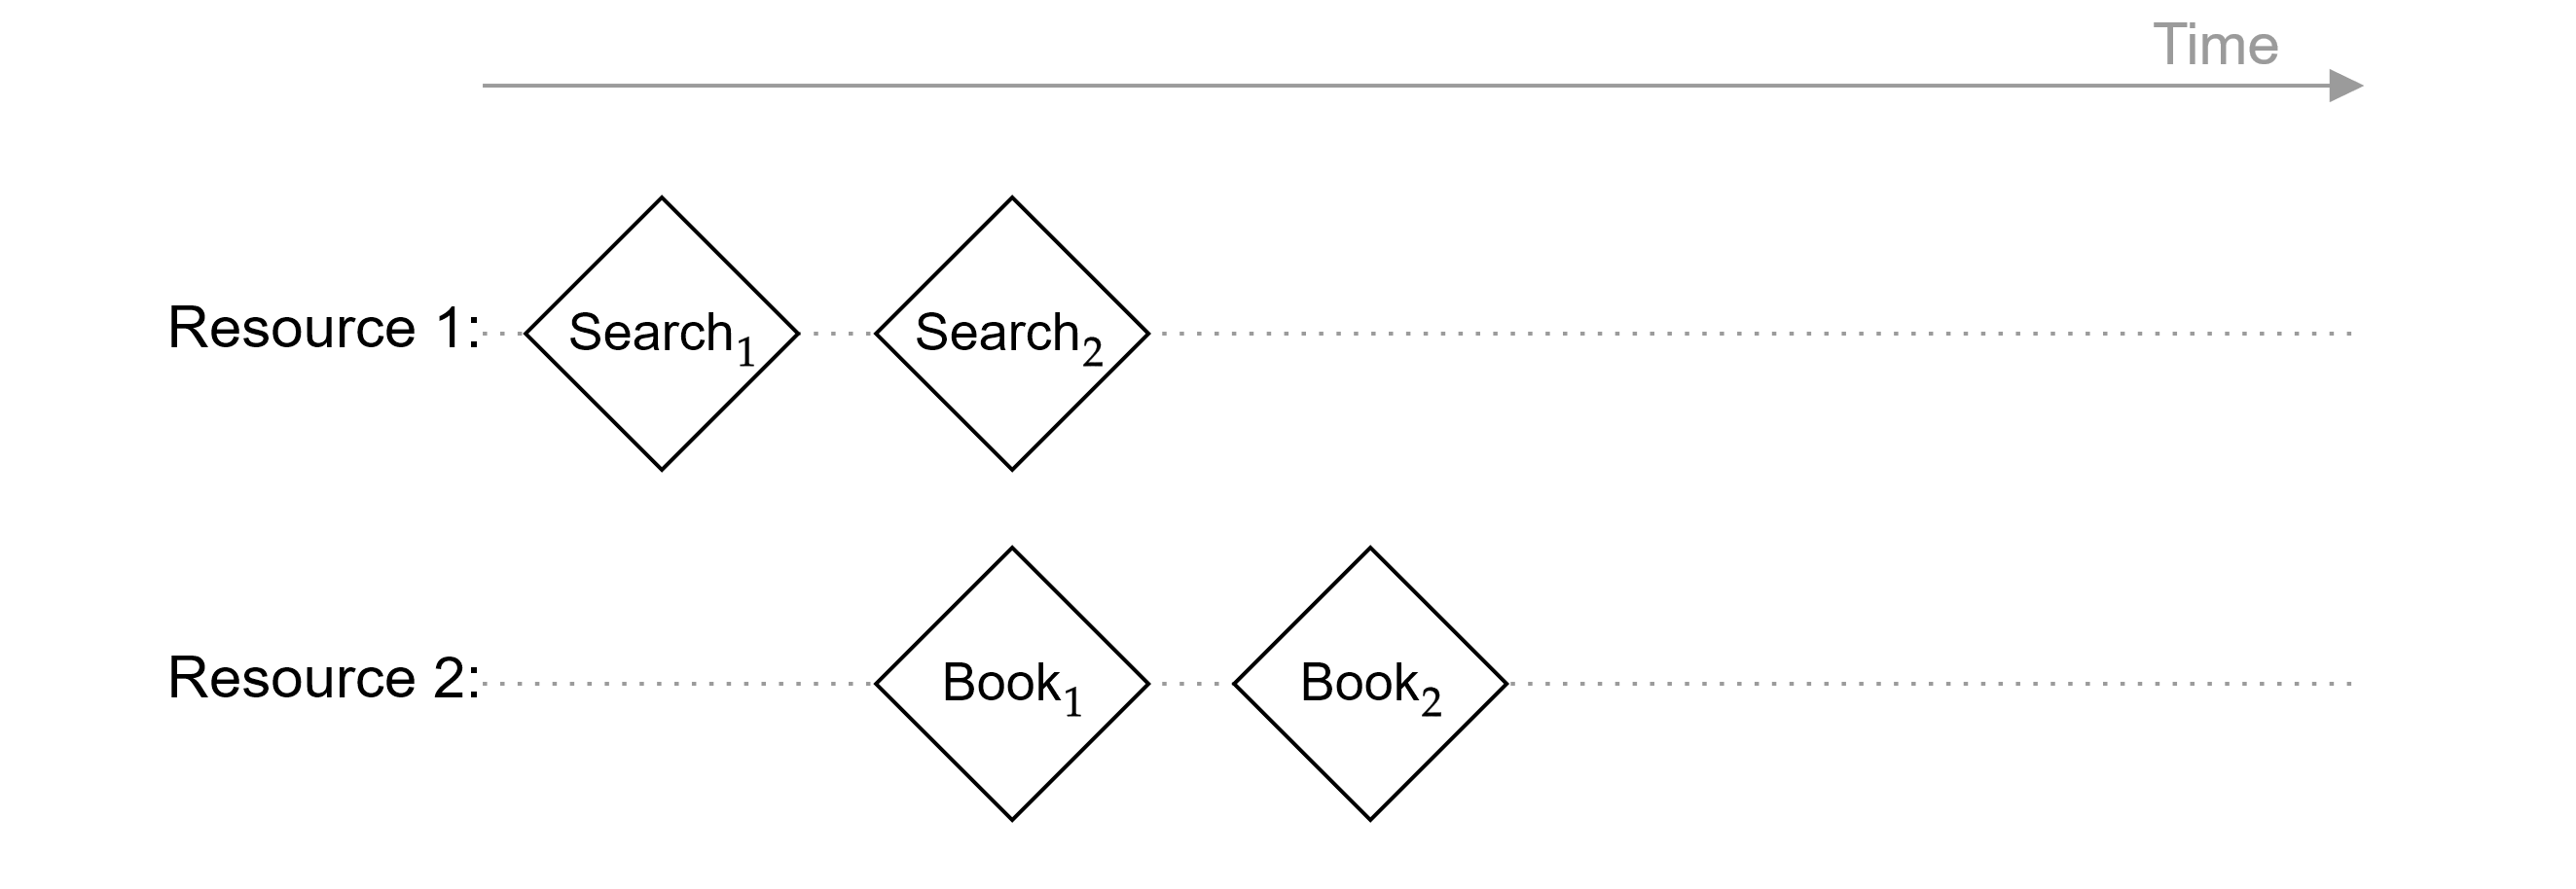
\includegraphics[width=1\textwidth]{./Sections/rpc_2/ppar_2.png}
    \caption{Searching and Booking flights in parallel}
\end{figure}
\noindent
In this case, once the first search is done, we can start booking the flight and search for the next flight in parallel.
